\documentclass{AeroStructure-ERJohnson}
\usepackage{arydshln}

\input crosslink.tex

%\usepackage{showframe}
\def\ShowFrameLinethickness{0.125pt}

\def\harp#1{\smash{\mathord{\buildrel{\lower3pt\hbox{$\scriptscriptstyle\rightharpoonup$}}\over{#1}}}}

\myexternaldocument{App_4P}
\myexternaldocument{Ch01_4P}
\myexternaldocument{Ch02_4P}
\myexternaldocument{Ch03_4P}
\myexternaldocument{Ch04_4P}
\myexternaldocument{Ch05_4P}
\myexternaldocument{Ch06_4P}
\myexternaldocument{Ch07_4P}
\myexternaldocument{Ch08_4P}
\myexternaldocument{Ch09_4P}
\myexternaldocument{Ch10_4P}
\myexternaldocument{Ch11_4P}
\myexternaldocument{Ch12_4P}
\myexternaldocument{Ch13_4P}
\myexternaldocument{Ch14_4P}
%\myexternaldocument{Ch15_4P}
\myexternaldocument{Ch16_4P}
\myexternaldocument{Ch17_4P}
\myexternaldocument{Ch18_4P}

\begin{document}

\mainmatter

%\hbox{~}\clearpage
\setcounter{page}{381}

\setcounter{chapter}{14}

\chapter{Direct stiffness method}\label{ch15}

Unit action states and unit displacement states are defined in the first section followed by an example to show how these definitions can be used to find flexibility and stiffness influence coefficients. To introduce the basic methods of matrix structural analysis, the analyses of structures modeled with linear elastic springs are presented in article \ref{sec15.2} to article \ref{sec15.6}. The objective is to illustrate the steps in the \textbf{direct stiffness method, }which is summarized in article \ref{sec15.7}. The approach followed here is based on chapters \ref{ch2}, \ref{ch3}, \ref{ch4}, and \ref{ch6} of Martin (1966).

\section{Physical interpretation of influence coefficients}\label{sec15.1}

\noindent
Consider the structural model of a cantilever wing with two degrees of freedom shown in figure \ref{fig15.1}. The generalized forces are denoted by $Q_{i}$ and the corresponding generalized displacements by $q_{i}$, $i=1,2$. Refer to the discussion in article \ref{sec5.2.1} and article \ref{sec5.2.2} on page \pageref{sec5.2.2}. The linear elastic response of the wing is determined from the matrix relations
{\def\thefigure{15.1}
\processfigure{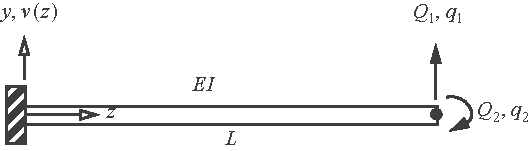
\includegraphics{Figure_15-1.pdf}}
{\caption{Two-degree-of-freedom model of the cantilever wing.\label{fig15.1}}}
}
\begin{align}\label{eq15.1}
\left[\begin{array}{@{}l@{}}
Q_{1} \\
Q_{2}
\end{array}\right]=\underbrace{\left[\begin{array}{@{}ll@{}} k_{11} & k_{12} \\k_{21} & k_{22}\end{array}\right]}_{[k]}\left[\begin{array}{@{}l@{}}q_{1} \\q_{2}\end{array}\right]\hspace*{1em}
\left[\begin{array}{@{}l@{}} q_{1} \\ q_{2} \end{array}\right]=\underbrace{\left[\begin{array}{@{}ll@{}} c_{11} & c_{12} \\ c_{21} & c_{22} \end{array}\right]}_{[c]}\left[\begin{array}{@{}l@{}} Q_{1} \\ Q_{2} \end{array}\right].
\end{align}
Elements $k_{i j}$ of the stiffness matrix are stiffness influence coefficients, and elements $c_{i j}$ of the flexibility matrix are flexibility influence coefficients. Matrices $[k]$ and $[c]$ are symmetric, and they are the inverse of one another;~i.e.,
\begin{align}\label{eq15.2}
[k]^{T}=[k] \quad[c]^{T}=[c] \quad[k][c]=[c][k]=[I].
\end{align}
The following definition of the stiffness influence coefficients is the basis of the unit displacement state (UDS) method:
\begin{quote}
\textit{The stiffness influence coefficient} ${\rm k}_{\rm ij}$ \textit{represents the generalized force at point} ${\rm i}$ \textit{in the direction} ${\rm q}_{\rm i}$ \textit{due to a unit generalized displacement} ${\rm q}_{\rm j}$, \textit{all other generalized displacements equal to zero.}
\end{quote}

\noindent For UDS 1 take the displacement vector $\left[\begin{array}{@{}l@{}}q_{1} \\q_{2}\end{array}\right]=\left[\begin{array}{@{}l@{}}1 \\0\end{array}\right]$, then the generalized forces from the first of eqs. (\ref{eq15.1}) are $\left[\begin{array}{@{}l@{}}Q_{1} \\Q_{2}\end{array}\right]=\left[\begin{array}{@{}l@{}}k_{11} \\k_{21}\end{array}\right] \cdot 1$. For UDS 1 the force vector is equal to the first column of the stiffness matrix. For UDS 2 take $\left[\begin{array}{@{}l@{}}q_{1} \\q_{2}\end{array}\right]=\left[\begin{array}{@{}l@{}}0 \\1\end{array}\right]$, then the generalized force vector is $\left[\begin{array}{@{}l@{}}Q_{1} \\Q_{2}\end{array}\right]=\left[\begin{array}{@{}l@{}}k_{12} \\k_{22}\end{array}\right] \cdot 1$. For UDS 2 the force vector is equal to the second column of the stiffness matrix. For the wing example the generalized force vectors in terms of the elements of the stiffness matrix are depicted in figure \ref{fig15.2}.

{\def\thefigure{15.2}
\processfigure{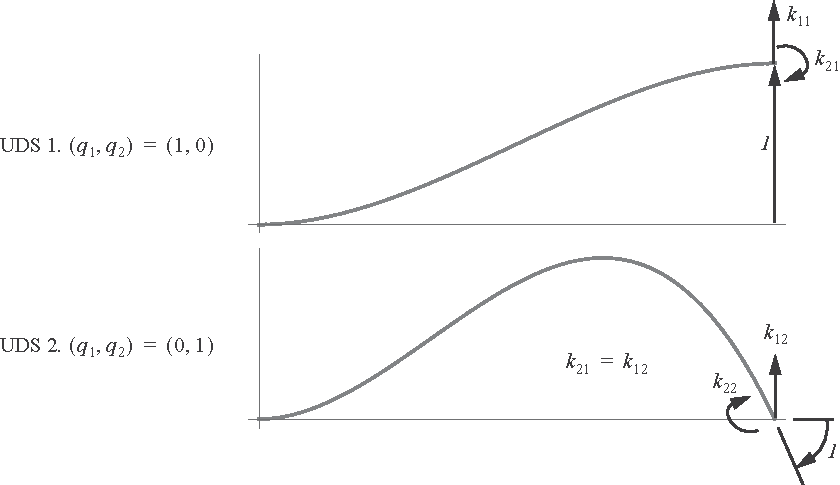
\includegraphics{Figure_15-2.pdf}
}{\caption{Generalized forces for the unit displacement states.\label{fig15.2}}}}


The following definition of the flexibility influence coefficients is the basis of the unit action state (UAS) method:

\begin{quote}
\textit{The flexibility influence coefficient ${\rm c}_{\rm ij}$ represents the generalized displacement at point ${\rm i}$ in the direction $\mathrm{Q}_\mathrm{i}$ due to a unit generalized force $\mathrm{Q}_\mathrm{j}$, all other generalized forces equal to zero.}
\end{quote}

For UAS 1 take the generalized force vector $\left[\begin{array}{@{}l@{}}Q_{1} \\Q_{2}\end{array}\right]=\left[\begin{array}{@{}l@{}}1 \\0\end{array}\right]$, then the generalized displacements from the second of eq.~(\ref{eq15.1}) are $\left[\begin{array}{@{}l@{}}q_{1} \\q_{2}\end{array}\right]=\left[\begin{array}{@{}l@{}}c_{11} \\c_{21}\end{array}\right] \cdot 1$. For UAS 1 the displacement vector is equal to the first column of the flexibility matrix. For UAS 2 take $\left[\begin{array}{@{}l@{}}Q_{1} \\Q_{2}\end{array}\right]=\left[\begin{array}{@{}l@{}}0 \\1\end{array}\right]$, then the generalized displacement vector is $\left[\begin{array}{@{}l@{}}q_{1} \\q_{2}\end{array}\right]=\left[\begin{array}{@{}l@{}}c_{12} \\c_{22}\end{array}\right] \cdot 1$. For UAS 2 the displacement vector is equal to the second column of the flexibility matrix. For the wing example the generalized displacement vectors in terms of the elements of the flexibility matrix are depicted in figure \ref{fig15.3}.

{\def\thefigure{15.3}
\processfigure{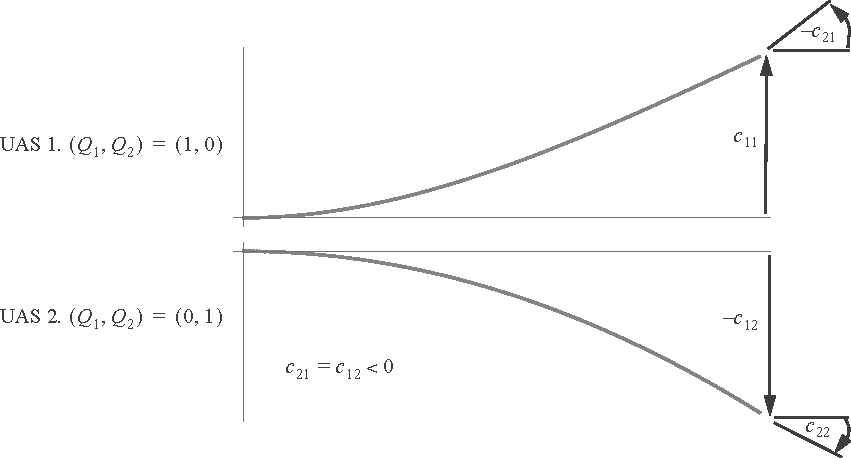
\includegraphics{Figure_15-3.pdf}
}{\caption{Generalized displacements for unit action states.\label{fig15.3}}}}

\begin{example}[Two springs in series restrained at one end.]\label{ex15.1}\setcounter{equation}{0}\def\theequation{\alph{equation}}Construct the flexibility influence matrix $[C]$ by the method of unit action states (UAS), and the stiffness influence matrix $[K]$, by the method of unit displacement states (UDS) for the two-degree-of freedom structural model shown in figure~\ref{fig15.4}. The model consists of two linear elastic springs in series with the left end fixed against translation. The left spring has stiffness $k_{a}$ and the right spring has stiffness $k_{b}$.

{\def\thefigure{15.4}
\begin{figure}[h]
\centering{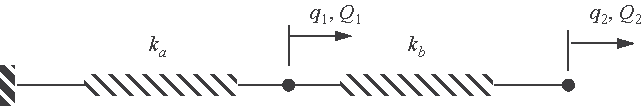
\includegraphics{Figure_15-4.pdf}}
\caption{Two linear elastic springs in series restrained against rigid body translation.\label{fig15.4}}
\end{figure}
}

The flexibility and stiffness matrix relations are of the form
\begin{align}\label{ex15.1a}
\left[\begin{array}{@{}l@{}}q_{1} \\q_{2}\end{array}\right]=\left[\begin{array}{@{}ll@{}}c_{11} & c_{12} \\c_{21} & c_{22}\end{array}\right]\left[\begin{array}{@{}l@{}}Q_{1} \\Q_{2}\end{array}\right] \quad\left[\begin{array}{@{}l@{}}Q_{1} \\Q_{2}\end{array}\right]=\left[\begin{array}{@{}ll@{}}k_{11} & k_{12} \\k_{21} & k_{22}\end{array}\right]\left[\begin{array}{@{}l@{}}q_{1} \\q_{2}\end{array}\right].
\end{align}

\pagebreak

\noindent\textbf{Solution.}

\noindent\textbf{UAS 1.}\enskip $Q_{1}=1$ and $Q_{2}=0$. The free body diagrams of the springs, with the spring forces assumed positive in tension, and of joints 1 and 2 are shown in figure \ref{fig15.4}.

\vspace*{-7pt}

{\def\thefigure{15.5}
\processfigure{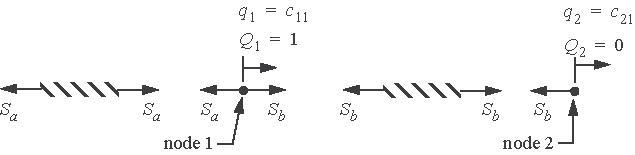
\includegraphics{Figure_15-5.pdf}
}{\caption{Unit action\break state~1. \phantom{0000}\label{fig15.5}}}}

\vspace*{-7pt}

Equilibrium at joints 1 and 2 gives
\begin{align}\label{ex15.1b}
-S_{a}+S_{b}+1=0 \quad S_{b}=0.
\end{align}
Therefore,
\begin{align}\label{ex15.1c}
S_{a}=1 \quad S_{b}=0.
\end{align}

The material laws for the linear elastic springs are
\begin{align}\label{ex15.1d}
S_{a}=k_{a} \Delta_{a} \quad S_{b}=k_{b} \Delta_{b}.
\end{align}
where $\Delta_{a}$ is the elongation of spring \textbf{a} and $\Delta_{b}$ is the elongation of spring \textbf{b}. Spring elongations are related to the nodal displacements by geometric compatibility, and for this example we have
\begin{align}\label{ex15.1e}
\Delta_{a}=q_{1} \quad \Delta_{b}=q_{2}-q_{1}.
\end{align}
\indent Thus, $1=k_{a} q_{1}$ and $0=k_{b}\left(q_{2}-q_{1}\right)$. Solve for the displacements to get
\begin{align}\label{ex15.1f}
q_{1}=\frac{1}{k_{a}}=c_{11} \quad q_{2}=\frac{1}{k_{a}}=c_{21}.
\end{align}

\noindent\textbf{UAS 2.}\enskip $Q_{1}=0$ and $Q_{2}=1$. The free body diagrams are shown in figure \ref{fig15.5}.

\vspace*{-7pt}

{\def\thefigure{15.6}
\processfigure{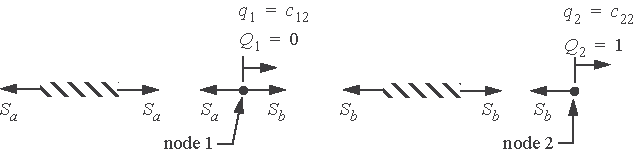
\includegraphics{Figure_15-6.pdf}
}{\caption{Unit action state 2.\label{fig15.6}}}}

\vspace*{-7pt}

\noindent Equilibrium at the joints gives
\begin{align}\label{ex15.1g}
-S_{a}+S_{b}=0 \quad-S_{b}+1=0.
\end{align}
Therefore,
\begin{align}\label{ex15.1h}
S_{a}=1 \quad S_{b}=1.
\end{align}

The material laws for each spring and the elongation-displacement relations give
\begin{align}\label{ex15.1i}
1=k_{a} q_{1} \quad 1=k_{b}\left(q_{2}-q_{1}\right).
\end{align}
Solve for the displacements to get
\begin{align}\label{ex15.1j}
q_{1}=\frac{1}{k_{a}}=c_{12} \quad q_{2}=\frac{1}{k_{a}}+\frac{1}{k_{b}}=c_{22}.
\end{align}

From the method of unit action states we have determined the flexibility matrix to be
\begin{align}\label{ex15.1k}
[C]=\left[\begin{array}{@{}cc@{}}\frac{1}{k_{a}} & \frac{1}{k_{a}} \\\frac{1}{k_{a}} & \left(\frac{1}{k_{a}}+\frac{1}{k_{b}}\right)\end{array}\right].
\end{align}
The flexibility matrix is symmetric, which it must be for a linear elastic structure by Maxwell's reciprocal theorem: See article \ref{sec5.1.2} on page \pageref{sec5.1.2}.

\noindent\textbf{UDS 1.}\enskip $q_{1}=1$ and $q_{2}=0$. From the material laws for each spring and the elongation-displacement relations we have
\begin{align}\label{ex15.1l}
S_{a}=k_{a} q_{1}=k_{a} \cdot 1=k_{a} \quad S_{b}=k_{b}\left(q_{2}-q_{1}\right)=k_{b}(-1)=-k_{b}.
\end{align}
Free body diagrams of the two joints are shown in figure \ref{fig15.6}.

{\def\thefigure{15.7}
\processfigure{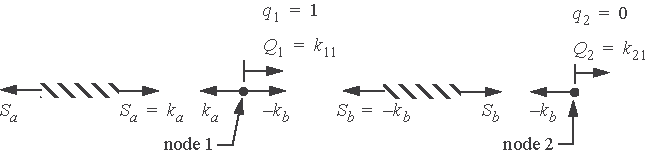
\includegraphics{Figure_15-7.pdf}
}{\caption{Unit~displace\-ment~state~1.\label{fig15.7}}}}

\noindent Equilibrium at the joints gives
\begin{align}\label{ex15.1m}
-S_{a}+S_{b}+Q_{1}=0 \quad{-}S_{b}+Q_{2}=0.
\end{align}
But $S_{a}=k_{a}$ and $S_{b}=-k_{b}$ for UDS 1. Also, we identify $Q_{1}=k_{11}$ and $Q_{2}=k_{21}$ for UDS 1. So
\begin{align}\label{ex15.1n}
k_{11}=k_{a}+k_{b} \quad k_{21}=-k_{b}.
\end{align}

\noindent\textbf{UDS 2.}\enskip $q_{1}=0$ and $q_{2}=1$. From the material laws for each spring and the elongation-displacement relations we have
\begin{align}\label{ex15.1o}
S_{a}=k_{a}(0)=0 \quad S_{b}=k_{b}(q_{2}-q_{1})=k_{b}(1-0)=k_{b}.
\end{align}
Free body diagrams of the two joints are shown in figure \ref{fig15.7}.

{\def\thefigure{15.8}
\processfigure{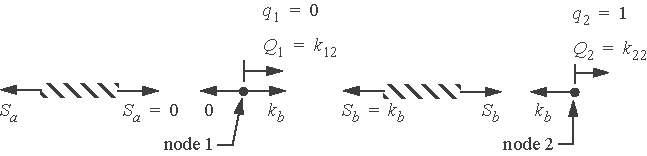
\includegraphics{Figure_15-8.pdf}
}{\caption{Unit~displace\-ment~state~2.\label{fig15.8}}}}

Nodal equilibrium gives
\begin{align}\label{ex15.1p}
-S_{a}+S_{b}+Q_{1}=0 \quad{-}S_{b}+Q_{2}=0.
\end{align}
But $S_{a}=0$ and $S_{b}=k_{b}$ for UDS 1. Also, we identify $Q_{1}=k_{12}$ and $Q_{2}=k_{22}$ for UDS 1. So
\begin{align}\label{ex15.1q}
k_{12}=-k_{b} \quad k_{22}=k_{b}.
\end{align}

Therefore, the stiffness matrix is
\begin{align}\label{ex15.1r}
[K]=\left[\begin{array}{@{}cc@{}}(k_{a}+k_{b}) & -k_{b} \\-k_{b} & k_{b}\end{array}\right].
\end{align}
The stiffness matrix is also symmetric, which was proved based on symmetry of the flexibility matrix. Refer to article \ref{sec5.2.2}.

Note that the matrix product
\[
[C][K]=\left[\begin{array}{@{}cc@{}}\frac{1}{k_{a}} & \frac{1}{k_{a}}\\ \frac{1}{k_{a}} & \left(\frac{1}{k_{a}}+\frac{1}{k_{b}}\right)\end{array}\right]
\left[\begin{array}{@{}cc@{}}(k_{a}+k_{b}) & -k_{b} \\-k_{b} & k_{b}\end{array}\right]=\left[\begin{array}{@{}cc@{}}\left(\frac{\left(k_{a}\,+\, k_{b}\right)}{k_{a}}-\frac{k_{b}}{k_{a}}\right) & \left(-\frac{k_{b}}{k_{a}}+\frac{k_{b}}{k_{a}}\right)\\ \left(\frac{\left(k_{a}\,+\, k_{b}\right)}{k_{a}}-k_{b}\left(\frac{1}{k_{a}}+\frac{1}{k_{b}}\right)\right) & \left(-\frac{k_{b}}{k_{a}}+k_{b}\left(\frac{1}{k_{a}}+\frac{1}{k_{b}}\right)\right)\end{array}\right]=\left[\begin{array}{@{}ll@{}}1 & 0 \\0 & 1\end{array}\right].
\]
That is, the product of flexibility matrix and the stiffness matrix is the identity matrix. In other words, the inverse of the flexibility matrix is the stiffness matrix.
\end{example}
\setcounter{equation}{2}

\section{Unrestrained structural stiffness matrix}\label{sec15.2}

The flexibility influence coefficients $c_{i j}$ are defined for a structure restrained against rigid body motion. However, it is not necessary to impose this rigid body constraint when forming the stiffness influence coefficients $k_{i j}$ of a structure. Specifying the generalized displacements in the method of unit displacement states encompasses both rigid body displacements and those causing deformation. Consider a single, linear elastic spring element with two-degrees-of-freedom (DOFs) connected between joints $i$ and \textit{j}, where integers $i \neq j$, as shown in figure~\ref{fig15.9}. Let $k$ denote the stiffness of the spring, which has dimensional units of \textit{F/L}.

{\def\thefigure{15.9}
\processfigure{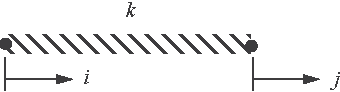
\includegraphics{Figure_15-9.pdf}
}{\caption{A two-degree-of-freedom spring element.\label{fig15.9}}}}


The unrestrained structural stiffness matrix is, in general, given by
\begin{align}\label{eq15.3}
\left[\begin{array}{@{}c@{}}Q_{i} \\Q_{j}\end{array}\right]=\left[\begin{array}{@{}ll@{}}k_{i i} & k_{i j} \\k_{j i} & k_{j j}\end{array}\right]\left[\begin{array}{@{}l@{}}q_{i} \\q_{j}\end{array}\right],
\end{align}
in which $i \neq j$. Free body diagrams of the joints and spring are shown in figure~\ref{fig15.10}. Equilibrium at the joints yields\vspace*{-12pt}
{\def\thefigure{15.10}
\processfigure[H]{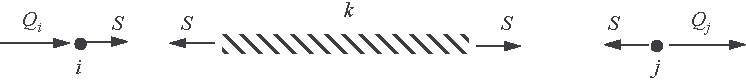
\includegraphics{Figure_15-10.pdf}
}{\caption{Free body diagram of the two-degree-of-freedom spring element.\label{fig15.10}}}}

\vspace*{-3pc}

\begin{align}\label{eq15.4}
Q_{i}+S=0 \quad Q_{j}-S=0.
\end{align}
The spring force is related to the nodal displacements by the material law
\begin{align}\label{eq15.5}
S=k\left(q_{j}-q_{i}\right).
\end{align}

\noindent\textbf{UDS 1.}\enskip $q_{i}=1$ and $q_{j}=0$. Therefore eq.~(\ref{eq15.5}) gives $S=-k \cdot 1$. Nodal equilibrium, eq.~(\ref{eq15.4}), and the matrix relation, eq.~(\ref{eq15.3}), give
\begin{align}\label{eq15.6}
Q_{i}=-(-k \cdot 1)=k_{i i} \quad Q_{j}=-k \cdot 1=k_{j i}.
\end{align}

\noindent\textbf{UDS 2.}\enskip $q_{i}=0$ and $q_{j}=1$. Therefore eq.~(\ref{eq15.5}) gives $S=k \cdot 1$. Nodal equilibrium, eq.~(\ref{eq15.4}), and the matrix relation, eq.~(\ref{eq15.3}), give
\begin{align}\label{eq15.7}
Q_{i}=-k \cdot 1=k_{i j} \quad Q_{j}=k \cdot 1=k_{j j}.
\end{align}
So that the unrestrained structural stiffness matrix is given by
\begin{align}\label{eq15.8}
[K]=\left[\begin{array}{@{}cc@{}}k & -k \\-k & k\end{array}\right]=k\left[\begin{array}{@{}cc@{}}1 & -1 \\-1 & 1\end{array}\right].
\end{align}

Note that the unrestrained structural stiffness matrix (\ref{eq15.8}) has the following properties:
\begin{enumerate}
  \item Matrix $[K]$ is symmetric (i.e., $[K]^{T}=[K]$).
  \item The sum of the column elements equals zero. $\sum\limits_{i\,=\,1}^2 k_{i j}=0$ for $j=1,2$. The vanishing of this sum results from $Q_{i}+Q_{j}=0$ for each UDS.
  \item The ${\it det}[K]=k^{2}-(-k)^{2}=0$. That is, the unrestrained structural stiffness matrix is \textit{singular}. This occurs because the structure is not restrained against rigid body translation in the horizontal direction.
Under the action of no external loads (i.e., $Q_{i}=0$ and $Q_{j}=0$), the structure can translate horizontally at a constant speed. Rigid body motion can be used to establish constraints between elements of the unrestrained structural stiffness matrix. For example, let $v$ denote the horizontal speed and let $t$ denote time, then
\begin{align}\label{eq15.9}
q_{i}=q_{j}=v t.
\end{align}
Equation (\ref{eq15.3}) gives
\begin{align}\label{eq15.10}
\left[\begin{array}{@{}l@{}}0 \\0\end{array}\right]=\left[\begin{array}{@{}ll@{}}k_{i i} & k_{i j} \\k_{j i} & k_{j j}\end{array}\right]\left[\begin{array}{@{}l@{}}v t \\v t\end{array}\right],
\end{align}
or
\begin{align}\label{eq15.11}
(k_{i i}+k_{i j}) q=0 \quad (k_{j i}+k_{j j}) q=0 \quad q=v t \neq 0.
\end{align}
Therefore, the constraints between elements of the unrestrained stiffness matrix are
\begin{align}\label{eq15.12}
k_{i i}+k_{i j}=0 \quad k_{j i}+k_{j j}=0.
\end{align}


\item Diagonal elements of $[K]$ are positive. This must be true based on physical grounds. If $Q_{i}>0$ and $q_{j}=0$, then we expect $q_{i}>0$. Thus, in the relation $Q_{i}=k_{i i} q_{i}$, the stiffness influence coefficient $k_{i i}>0$.
\end{enumerate}

\section{Assembly of unrestrained structural stiffness matrices}\label{sec15.3}
Consider the construction of the 3X3 stiffness matrix for the unrestrained structure shown in figure \ref{fig15.11} given the generic stiffness matrix of the spring element from eq.~(\ref{eq15.8}).


{\def\thefigure{15.11}
\begin{figure}[h]
\centering{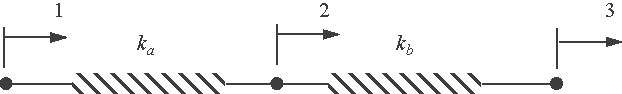
\includegraphics{Figure_15-11.pdf}}
\caption{Unrestrained structure composed of two springs in series.\label{fig15.11}}
\end{figure}
}

Using the results from eq.~(\ref{eq15.8}) for each separate spring element, we can write the following results
\begin{align}
\raisebox{-10pt}{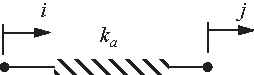
\includegraphics{Unnumbered_Fig_Ch15_Eqn_15-13.pdf}}\qquad& \left[\begin{array}{@{}l@{}}Q_{i} \\Q_{j}\end{array}\right]=\left[\begin{array}{@{}cc@{}}k_{a} & -k_{a} \\-k_{a} & k_{a}\end{array}\right]\left[\begin{array}{@{}l@{}}q_{i} \\q_{j}\end{array}\right] \label{eq15.13}\\[6pt]
\raisebox{-10pt}{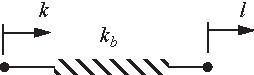
\includegraphics{Unnumbered_Fig_Ch15_Eqn_15-14.pdf}}\qquad&\left[\begin{array}{@{}l@{}} Q_{k} \\ Q_{l}\end{array}\right]=\left[\begin{array}{@{}cc@{}}k_{b} & -k_{b} \\-k_{b} & k_{b}\end{array}\right]\left[\begin{array}{@{}l@{}}q_{k} \\q_{l}\end{array}\right].\label{eq15.14}
\end{align}
\textit{Assembly} of the individual spring element stiffness matrices is accomplished by displacement continuity at the joints and equilibrium at the joints. Displacement continuity requires
\begin{align}\label{eq15.15}
q_{i}=q_{1} \quad q_{j}=q_{k}=q_{2} \quad q_{l}=q_{3}.
\end{align}
A free body diagram of the structure is shown below.

{\def\thefigure{15.12}
\processfigure{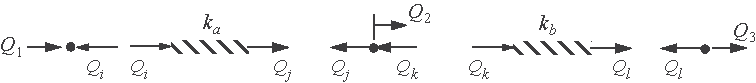
\includegraphics{Figure_15-12.pdf}
}{\caption{Free body diagram of the two springs in series.\label{fig15.12}}}}

\noindent Equilibrium at the three joints requires
\begin{align}\label{eq15.16}
Q_{1}=Q_{i} \quad Q_{2}=Q_{j}+Q_{k} \quad Q_{3}=Q_{l}.
\end{align}
Substitute for the displacements of the individual spring elements in eqs. (\ref{eq15.13}) and (\ref{eq15.14}) the structural displacements in eqs. (\ref{eq15.15}). Then substitute, in turn, these results into the nodal equilibrium eq.~(\ref{eq15.16}) to eliminate individual spring forces $Q_{i}, Q_{j}, Q_{k}, \text{ and } Q_{l}$. We\vspace*{-3pt} get
\begin{align}\label{eq15.17}
\begin{gathered}Q_{1}=k_{a} q_{1}-k_{a} q_{2} \\Q_{2}=-k_{a} q_{1}+k_{a} q_{2}+k_{b} q_{2}-k_{b} q_{3} \\Q_{3}=-k_{b} q_{2}+k_{b} q_{3}\end{gathered},
\end{align}
Write eq.~(\ref{eq15.17}) in matrix\vspace*{-3pt} form
\begin{align}\label{eq15.18}
\left[\begin{array}{@{}l@{}}Q_{1} \\Q_{2} \\Q_{3}\end{array}\right]=\left[\begin{array}{@{}ccc@{}}k_{a} & -k_{a} & 0 \\ -k_{a} & (k_{a}+k_{b}) & -k_{b} \\ 0 & -k_{b} & k_{b}\end{array}\right]\left[\begin{array}{@{}l@{}}q_{1} \\q_{2} \\q_{3}\end{array}\right].
\end{align}
Hence, the \textit{unrestrained structural stiffness matrix}\vspace*{-3pt} is
\begin{align}\label{eq15.19}
[K]=\left[\begin{array}{@{}ccc@{}}k_{a} & -k_{a} & 0 \\ -k_{a} & (k_{a}+k_{b}) & -k_{b} \\0 & -k_{b} & k_{b}\end{array}\right].
\end{align}

\removelastskip

Note the following properties of the unrestrained structural stiffness matrix in eq.~(\ref{eq15.19}):
\begin{enumerate}
\item The matrix is symmetric, or $[K]^{T}=[K]$.
\item Using a co-factor expansion by the third column, the determinate of the matrix is computed as follows:
\begin{gather*}
\operatorname{\it det}[K]=(0) \operatorname{\it det}\left[\begin{array}{@{}cc@{}}-k_{a} & (k_{a}+k_{b}) \\ 0 & -k_{b}\end{array}\right]-(-k_{b}) \operatorname{\it det}\left[\begin{array}{@{}cc@{}}k_{a} & -k_{a} \\ 0 & -k_{b}\end{array}\right]+\left(k_{b}\right) \operatorname{\it det}\left[\begin{array}{@{}cc@{}}k_{a} & -k_{a} \\-k_{a} & (k_{a}+k_{b})\end{array}\right] \\ \operatorname{\it det}[K]=0-k_{a} k_{b}^{2}+(k_{b})[k_{a}(k_{a}+k_{b})-k_{a}^{2}]=-k_{a} k_{b}^{2}+k_{a} k_{b}^{2}=0.
\end{gather*}
Since the determinate is zero, the matrix is singular. The unrestrained structural stiffness matrix is singular because rigid body translation is not restrained.

\item The sum of the column elements is zero. $\sum\limits_{i\,=\,1}^3 k_{i j}=0$ for $j=1,2,3$.

\item Diagonal elements are positive $k_{i i}>0$.
\end{enumerate}

Of course, we could have used the method of unit displacement states to determine the unrestrained structural stiffness matrix (\ref{eq15.19}) for the two springs in series rather than the assembly procedure given above.

Another way to obtain the unrestrained structural stiffness matrix is to first expand the element unrestrained stiffness matrices to size 3X3 by adding rows and columns of zeros, and then add the 3X3 element stiffness matrices. For spring element stiffness matrix given by eq.~(\ref{eq15.13}), displacement compatibility, eq.~(\ref{eq15.15}), identifies $q_{i}=q_{1}$ and $q_{j}=q_{2}$. That is, columns one and two of the element stiffness matrix are associated with global degrees of freedom one and two. We write the element stiffness matrix\vspace*{-3pt} as
\begin{align}\label{eq15.20}
\left[K_{a}\right]=
\begin{array}{@{}l@{}}
{\begin{array}{@{}l@{}}\hspace*{8pt}  q_{1} \hspace*{18pt} q_{2} \hspace*{10pt} q_{3} \end{array}}\\[4pt]
\left[\begin{array}{@{}ccc@{}}
k_{a} & -k_{a} & 0 \\
-k_{a} & k_{a} & 0 \\
0 & 0 & 0
\end{array}
\right]
\end{array}.
\end{align}
The global degrees of freedom are written above the appropriate columns of the expanded element stiffness matrix in eq.~(\ref{eq15.20}) to aid in keeping the order of the element columns consistent with the ordering\vadjust{\pagebreak} of the global \nobreak{displacements}. For the spring element stiffness matrix given by eq.~(\ref{eq15.14}), displacement compatibility, eq.~(\ref{eq15.15}), identifies $q_{k}=q_{2}$ and $q_{l}=q_{3}$. That is, columns one and two of the element stiffness matrix are associated with global degrees of freedom two and three. We write the element stiffness matrix as
\begin{align}\label{eq15.21}
\left[K_{b}\right]=
\begin{array}{@{}l@{}}
{\begin{array}{@{}l@{}}\ q_{1} \hspace*{10pt} q_{2} \hspace*{18pt} q_{3} \end{array}}\\[4pt]
\left[\begin{array}{@{}ccc@{}}
0 & 0 & 0 \\0 & k_{b} & -k_{b} \\0 & -k_{b} & k_{b}
\end{array}\right]
\end{array}.
\end{align}
Note that the only non-zero elements in the expanded element stiffness matrix (\ref{eq15.21}) are in rows and columns two and three. Since matrices (\ref{eq15.20}) and (\ref{eq15.21}) are of the same dimensions we can add them to get the unrestrained stiffness matrix of the structure; i.e.,
\begin{align}\label{eq15.22}
[K]=\left[K_{a}\right]+\left[K_{b}\right]=
\begin{array}{@{}l@{}}
{\begin{array}{@{}l@{}}\hspace*{10pt}  q_{1} \hspace*{25pt} q_{2} \hspace*{27pt} q_{3} \end{array}}\\[4pt]
\left[\begin{array}{@{}ccc@{}}
k_{a} & -k_{a} & 0 \\
-k_{a} &(k_{a}+k_{b}) & -k_{b} \\
0 & -k_{b} & k_{b}
\end{array}\right]
\end{array}.
\end{align}
The unrestrained structural stiffness matrix in eq.~(\ref{eq15.22}) is the same as the matrix in eq.~(\ref{eq15.19}). Thus, the superposition of individual element stiffness matrices to obtain the unrestrained structural stiffness matrix is equivalent to imposing displacement compatibility and equilibrium at the joints.

\section{Prescribed nodal displacements and forces}\label{sec15.4}
At a joint we can prescribe either the displacement or the corresponding force, \textit{but not both}. Consider the unrestrained structure of the last section in which we prescribe the values of the displacement $q_{1}$, force $Q_{2}$, and force $Q_{3}$. That is, nodal values of $q_{1}, Q_{2}, \text{ and } Q_{3}$ are known, and nodal values of $Q_{1}, q_{2}, \text{ and } q_{3}$ are unknown. Nodal forces $Q_{2}, \text{ and } Q_{3}$ are the applied loads, and nodal force $Q_{1}$ is a reactive force, or support reaction. Nodal displacements $q_{2}, \text{ and } q_{3}$ are the unknown, or active, displacement degrees of freedom. We partition the unrestrained stiffness matrix given in eq.~(\ref{eq15.22}) by drawing lines between rows and columns to separate active and reactive nodal variables. In this example, we partition row 1 and column 1 as
\begin{align}\label{eq15.23}
\left[\begin{array}{@{}c@{}}Q_{1} \\\hdashline Q_{2} \\Q_{3}\end{array}\right]=\left[{\arraycolsep=7pt\begin{array}{c:cc}k_{a} & -k_{a} & 0 \\\hdashline-k_{a} & (k_{a}+k_{b}) & -k_{b} \\0 & -k_{b} & k_{b}\end{array}}\right]\left[\begin{array}{@{}l@{}}q_{1} \\\hdashline q_{2} \\q_{3}\end{array}\right].
\end{align}
Now rearrange the order of the equations and the order of the displacements in eq.~(\ref{eq15.23}). The equations for the applied loads $Q_{2}, \text{ and } Q_{3}$ are moved to correspond with rows one and two, and the reactive force equation for $Q_{1}$ is put in row three. Simultaneously, the unknown displacements $q_{2}, \text{ and } q_{3}$ are ordered such that they appear in columns one and two, and the prescribed displacement $q_{1}$ appears in column three. The equations in matrix form now read as
\begin{align}\label{eq15.24}
\left[\begin{array}{@{}c@{}}Q_{2} \\Q_{3} \\\hdashline Q_{1}\end{array}\right]=\left[{\arraycolsep=7pt\begin{array}{cc:c}(k_{a}+k_{b}) & -k_{b} & -k_{a} \\-k_{b} & k_{b} & 0 \\\hdashline-k_{a} & 0 & k_{a}\end{array}}\right]\left[\begin{array}{@{}l@{}}q_{2} \\q_{3} \\q_{1}\end{array}\right].
\end{align}
The rearranged stiffness matrix is
\begin{align}\label{eq15.25}
[K]=
\begin{array}{@{}l@{}}
{\begin{array}{@{}l@{}}\hspace*{20pt}  q_{2} \hspace*{32pt} q_{3} \hspace*{22pt} q_{1} \end{array}}\\[4pt]
\left[{\arraycolsep=7pt\begin{array}{@{}cc:c@{}}
(k_{a}+k_{b}) & -k_{b} & -k_{a} \\-k_{b} & k_{b} & 0 \\\hdashline-k_{a} & 0 & k_{a}\end{array}}\right]
\end{array}.
\end{align}
In terms of matrix algebra, the unrestrained stiffness matrix in eq.~(\ref{eq15.22}) was rearranged to the matrix in eq.~(\ref{eq15.25}) by the following four-step sequence: First interchange elements in rows 1 and 3. Second, interchange elements in columns 1 and 3. Third, interchange elements in rows 1 and 2. Fourth, interchange elements in columns 1 and 2.

Let the vector of unknown displacement degrees of freedom be denoted by $\{q_{\alpha}\}$, the vector of prescribed displacements by $\{q_{\beta}\}$, the vector of applied forces by $\{Q_{\alpha}\}$, and the vector of reactive forces by $\{Q_{\beta}\}$. In the example of this and the last section these vectors are
\begin{align}\label{eq15.26}
\{q_{\alpha}\}=\left[\begin{array}{@{}l@{}}q_{2} \\q_{3}\end{array}\right] \quad\{q_{\beta}\}=\left[q_{1}\right] \quad\{Q_{\alpha}\}=\left[\begin{array}{@{}l@{}}Q_{2} \\Q_{3}\end{array}\right] \quad\{Q_{\beta}\}=\left[Q_{1}\right].
\end{align}
The unrestrained structural stiffness matrix is rearranged to separate unknown and known nodal variables. In general, this partitioned matrix is written in the form
\begin{align}\label{eq15.27}
[K]= \left[\begin{array}{@{}cc@{}}{[K_{\alpha \alpha}]} & {[K_{\alpha \beta}]} \\[4pt]
{[K_{\beta \alpha}]} & {\left[K_{\beta \beta}\right]}\end{array}\right].
\end{align}
For the example in this and the last section, a comparison to the matrix in eq.~(\ref{eq15.25}) gives the submatrices in eq.~(\ref{eq15.27}) as
\begin{align}\label{eq15.28}
[K_{\alpha \alpha}]=\left[\begin{array}{@{}cc@{}}(k_{a}+k_{b}) & -k_{b} \\-k_{b} & k_{b}\end{array}\right] \quad[K_{\alpha \beta}]=\left[\begin{array}{@{}c@{}}-k_{a} \\0\end{array}\right] \quad[K_{\beta \alpha}]=\left[\begin{array}{@{}c@{}}-k_{a} 0\end{array}\right] \quad\left[K_{\beta \beta}\right]=\left[k_{a}\right].
\end{align}
The matrix equations for the structure in partitioned form are now written as
\begin{align}\label{eq15.29}
\left[\begin{array}{@{}l@{}}\{Q_{\alpha}\} \\\{Q_{\beta}\}\end{array}\right]=\left[\begin{array}{@{}l@{}}{[K_{\alpha \alpha}][K_{\alpha \beta}]} \\[4pt] {[K_{\beta \alpha}]\left[\begin{array}{@{}l@{}}K_{\beta \beta}\end{array}\right]}\end{array}\right]\left[\begin{array}{@{}l@{}}\{q_{\alpha}\} \\\{q_{\beta}\}\end{array}\right].
\end{align}
Submatrix $\left[K_{\alpha\alpha}\right]$ is called the \textbf{restrained structural stiffness matrix}. It is a square, symmetric matrix. For the example of this section it is seen from eq.~(\ref{eq15.28}) that the restrained stiffness matrix is 2X2, and its determinate is positive (i.e., $\operatorname{\it det}\left[K_{\alpha\alpha}\right]=k_{a} k_{b}>0$). The restrained structural stiffness matrix is nonsingular if the prescribed nodal displacements are sufficient to prevent rigid body motion of the structure. The restrained structural stiffness matrix for this example was determined by the method of unit displacement states in example 15.1. See eq.(\textbf{r)}. The submatrix $\left[K_{\beta \beta}\right]$ is, in general, square and symmetric. For the example in this section, eq.~(\ref{eq15.28}) shows $\left[K_{\beta \beta}\right]$ is 1X1. The off-diagonal submatrices are, in general, rectangular, but they satisfy the relationship
\begin{align}\label{eq15.30}
[K_{\beta \alpha}]=[K_{\alpha \beta}]^{T}.
\end{align}
\section{Solution for the unknown nodal variables}\label{sec15.5}

Multiply out the matrix equations (\ref{eq15.29}) following the ordinary matrix product formula to get
\begin{align}\label{eq15.31}
\{Q_{\alpha}\} &=[K_{\alpha\alpha}]\{q_{\alpha}\}+[K_{\alpha \beta}]\{q_{\beta}\}\\
\label{eq15.32}
\{Q_{\beta}\} &=[K_{\beta \alpha}]\{q_{\alpha}\}+[K_{\beta \beta}]\{q_{\beta}\}.
\end{align}
Since the applied load vector $\{Q_{\alpha}\}$ and the prescribed displacement vector $\{q_{\beta}\}$ are known, solve eq.~(\ref{eq15.31}) for the unknown nodal displacement vector to get
\begin{align}\label{eq15.33}
\{q_{\alpha}\}=[K_{\alpha \alpha}]^{-1}\{Q_{\alpha}\}-[K_{\alpha \alpha}]^{-1}[K_{\alpha \beta}]\{q_{\beta}\}.
\end{align}

Continuing with the example of the last two sections, the restrained structural stiffness matrix is given in first of eqs. (\ref{eq15.28}). Its inverse can be computed from
\[
[K_{\alpha \alpha}]^{-1}=\frac{\operatorname{\it adj}[K_{\alpha \alpha}]}{\operatorname{\it det}[K_{\alpha \alpha}]}.
\]
where $\operatorname{\it adj}[K_{\alpha \alpha}]$ is the \textit{adjoint matrix}. The adjoint matrix\footnote{Many determinates must be evaluated to compute the adjoint matrix. For large matrices, evaluating many determinates is computationally inefficient. Other, more efficient methods to solve large linear systems of equations are used in numerical
algorithms.} is the transpose of the matrix of co-factors of matrix $[K_{\alpha \alpha}]$. For the 2X2 restrained structural stiffness matrix (\ref{eq15.28})$_1$ in this example, the adjoint matrix is simple to compute. It is
\begin{align}\label{eq15.34}
\operatorname{\it adj}[K_{\alpha \alpha}]=
\left[\begin{array}{@{}lc@{}}k_{b} & k_{b} \\ k_{b} & (k_{a}+k_{b})\end{array}\right]^{T}=\left[\begin{array}{@{}lc@{}}k_{b} & k_{b} \\ k_{b} & (k_{a}+k_{b})\end{array}\right].
\end{align}
Hence, the inverse matrix is
\begin{align}\label{eq15.35}
\left[K_{\alpha \alpha}\right]^{-1}=\frac{1}{(k_{a}+k_{b}) k_{b}-k_{b}^{2}}\left[\begin{array}{@{}cc@{}}k_{b} & k_{b} \\ k_{b} & (k_{a}+k_{b})\end{array}\right]=\left[\begin{array}{@{}cc@{}}\frac{1}{k_{a}} & \frac{1}{k_{a}} \\ \frac{1}{k_{a}} & \left(\frac{1}{k_{a}}+\frac{1}{k_{b}}\right)\end{array}\right].
\end{align}
Of course, the inverse of the restrained structural stiffness matrix is recognized as the flexibility matrix. Equation (\ref{eq15.35}) was also obtained by the method of unit action state in example \ref{ex15.1} eq. (\textbf{k}). Continuing with the computations indicated in eq.~(\ref{eq15.33}) for this example, we have
\begin{gather}
\left[\begin{array}{@{}l@{}}q_{2} \\q_{3}\end{array}\right]=\left[\begin{array}{@{}cc@{}}\frac{1}{k_{a}} & \frac{1}{k_{a}} \\ \frac{1}{k_{a}} & \left(\frac{1}{k_{a}}+\frac{1}{k_{b}}\right)\end{array}\right]\left[\begin{array}{@{}l@{}}Q_{2} \\Q_{3}\end{array}\right]-\left[\begin{array}{@{}cc@{}}\frac{1}{k_{a}} & \frac{1}{k_{a}} \\ \frac{1}{k_{a}} & \left(\frac{1}{k_{a}}+\frac{1}{k_{b}}\right)\end{array}\right]\left[\begin{array}{@{}c@{}}-k_{a} \\0\end{array}\right]\left[q_{1}\right] \nonumber\\ \left[\begin{array}{@{}l@{}} q_{2} \\ q_{3}\end{array}\right]=\left[\begin{array}{@{}cc@{}}\frac{1}{k_{a}} & \frac{1}{k_{a}} \\ \frac{1}{k_{a}} & \left(\frac{1}{k_{a}}+\frac{1}{k_{b}}\right)\end{array}\right]\left[\begin{array}{@{}l@{}}Q_{2} \\Q_{3}\end{array}\right]-\left[\begin{array}{@{}c@{}}-1 \\-1\end{array}\right]\left[q_{1}\right]=\left[\begin{array}{@{}c@{}}\frac{\left(Q_{2}\,+\,Q_{3}\right)}{k_{a}}+q_{1} \\\frac{Q_{2}}{k_{a}}+\left(\frac{1}{k_{b}}+\frac{1}{k_{a}}\right) Q_{3}+q_{1}\end{array}\right].\label{eq15.36}
\end{gather}
Equation (\ref{eq15.36}) is the solution for the unknown nodal displacements.

To find the reactive nodal force vector, substitute the solution for the active nodal displacement vector from eq.~(\ref{eq15.33}) into eq.~(\ref{eq15.32}) to get
\begin{align}\label{eq15.37}
\{Q_{\beta}\}=[K_{\beta \alpha}]\left\{[K_{\alpha \alpha}]^{-1}\{Q_{\alpha}\}-\left[K_{\alpha \alpha}\right]^{-1}[K_{\alpha \beta}]\{q_{\beta}\}\right\}+\left[K_{\beta \beta}\right]\{q_{\beta}\}.
\end{align}
Multiply the matrix products and collect terms in the prescribed nodal displacement vector to get
\begin{align}\label{eq15.38}
\{Q_{\beta}\}=[K_{\beta \alpha}][K_{\alpha \alpha}]^{-1}\{Q_{\alpha}\}+\left\{\left[K_{\beta \beta}\right]-[K_{\beta \alpha}][K_{\alpha \alpha}]^{-1}[K_{\alpha \beta}]\right\}\{q_{\beta}\}.
\end{align}
\indent Let's evaluate eq.~(\ref{eq15.38}) for the example problem. From eqs. (\ref{eq15.28}) and (\ref{eq15.35})
\begin{align}\label{eq15.39}
Q_{1}=\left[\begin{array}{@{}ll@{}}-k_{a} & 0\end{array}\right]\left[\begin{array}{@{}cc@{}}\frac{1}{k_{a}} & \frac{1}{k_{a}} \\ \frac{1}{k_{a}} & \left(\frac{1}{k_{a}}+\frac{1}{k_{b}}\right)\end{array}\right]\left[\begin{array}{@{}l@{}}Q_{2} \\Q_{3}\end{array}\right]+\left\{k_{a}-\left[\begin{array}{@{}ll@{}}-k_{a} & 0\end{array}\right]\left[\begin{array}{@{}cc@{}}\frac{1}{k_{a}} & \frac{1}{k_{a}} \\ \frac{1}{k_{a}} & \left(\frac{1}{k_{a}}+\frac{1}{k_{b}}\right)\end{array}\right]\left[\begin{array}{@{}c@{}}-k_{a} \\0\end{array}\right]\right\} q_{1}.
\end{align}

\pagebreak

\noindent Performing some of the matrix products, we get
\begin{align}\label{eq15.40}
Q_{1}=\left[\begin{array}{@{}ll@{}}-1 & -1\end{array}\right]\left[\begin{array}{@{}l@{}}Q_{2} \\Q_{3}\end{array}\right]+\left\{k_{a}-k_{a}\right\} q_{1}.
\end{align}
This last matrix expression is equivalent to the scalar equation
\begin{align}\label{eq15.41}
Q_{1}=-Q_{2}-Q_{3}.
\end{align}
The result (\ref{eq15.41}) for the reactive nodal force is as expected from overall equilibrium of the structure shown in figure \ref{fig15.11}.

\section{Stress matrix}\label{sec15.6}

The stress matrix is a matrix that directly yields the internal forces or stresses in an element in terms of the nodal displacements. Consider a typical spring element between joints $i$ and $j$ as shown in figure \ref{fig15.13}. From the overall solution for the structural response, the nodal displacement vector $\{q_{\alpha}\}$ is determined. Hence, the actual nodal displacements $q_{i}$ and $q_{j}$ for the typical spring element are known. Define a vector of \textit{equivalent nodal forces} as the element stiffness matrix times the known nodal displacement vector, or
{\def\thefigure{15.13}
\processfigure{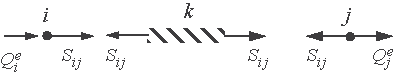
\includegraphics{Figure_15-13.pdf}
}{\caption{Typical spring element and equivalent joint forces.\label{fig15.13}}}}
\begin{align}\label{eq15.42}
\left[\begin{array}{@{}c@{}}Q_{i} \\Q_{j}\end{array}\right]^{e} \equiv\left[\begin{array}{@{}cc@{}}k & -k \\-k & k\end{array}\right]\left[\begin{array}{@{}l@{}}q_{i} \\q_{j}\end{array}\right].
\end{align}
These equivalent nodal forces are not the actual forces at the joints, so they are fictitious. From this equation, the equivalent nodal forces at the joint are
\begin{align}\label{eq15.43}
Q_{i}^{e}=\left[\begin{array}{@{}ll@{}}k & -k\end{array}\right]\left[\begin{array}{@{}l@{}}q_{i} \\q_{j}\end{array}\right] \quad Q_{j}^{e}=\left[\begin{array}{@{}ll@{}}-k & k\end{array}\right]\left[\begin{array}{@{}l@{}}q_{i} \\q_{j}\end{array}\right].
\end{align}
From the free body diagram shown in figure \ref{fig15.13}, the spring force $S_{i j}$ is related to the equivalent nodal forces by
\begin{align}\label{eq15.44}
Q_{i}^{e}=-S_{i j} \quad Q_{j}^{e}=S_{i j}.
\end{align}
Substitute eqs. (\ref{eq15.43}) into (\ref{eq15.44}) to eliminate the equivalent nodal forces to find that both of eqs. (\ref{eq15.44}) lead to the same expression for the spring element force. The result is
\begin{align}\label{eq15.45}
S_{i j}=\left[\begin{array}{@{}ll@{}}-k & k\end{array}\right]\left[\begin{array}{@{}l@{}}q_{i} \\q_{j}\end{array}\right]=[S]\left[\begin{array}{@{}l@{}}q_{i} \\q_{j}\end{array}\right],
\end{align}
where $[S]$ is the stress matrix for the spring element given by
\begin{align}\label{eq15.46}
[S]=\left[\begin{array}{@{}ll@{}}-k & k\end{array}\right].
\end{align}

For the example problem, the stress matrix for the spring between joints 1 and 2 is $\left[-k_{a}\ k_{a}\right]$. Then, force in the spring element is
\[
S_{12}=\left[\begin{array}{@{}ll@{}}-k_{a} & k_{a}\end{array}\right]\left[\begin{array}{@{}l@{}}q_{1} \\q_{2}\end{array}\right].
\]
From eq.~(\ref{eq15.36}), the displacement at joint 2 is
\[
q_{2}=\left(\frac{Q_{2}}{k_{a}}+\frac{Q_{3}}{k_{a}}\right)+q_{1}.
\]
Hence, the force in the spring element between joints 1 and 2 is
\[
S_{12}=-k_{a} q_{1}+k_{a} q_{2}=-k_{a} q_{1}+k_{a}\left[\left(\frac{Q_{2}}{k_{a}}+\frac{Q_{3}}{k_{a}}\right)+q_{1}\right]=Q_{2}+Q_{3}.
\]
The stress matrix for the spring between joints 2 and 3 is $\left[\begin{array}{@{}ll@{}}-k_{b} & k_{b}\end{array}\right]$. Then the force in this spring element is
\[
S_{23}=\left[\begin{array}{@{}ll@{}}-k_{b} & k_{b}\end{array}\right]\left[\begin{array}{@{}l@{}}q_{2} \\q_{3}\end{array}\right].
\]
Substitute the solution for the nodal displacements from eq.~(\ref{eq15.36}) into previous equation to get
\[
S_{23}=\left[\begin{array}{@{}ll@{}}-k_{b} & k_{b}\end{array}\right]\left[\begin{array}{@{}cc@{}}\frac{1}{k_{a}} & \frac{1}{k_{a}} \\[5pt] \frac{1}{k_{a}} & \left(\frac{1}{k_{a}}+\frac{1}{k_{b}}\right)\end{array}\right]
\left[\begin{array}{@{}l@{}}Q_{2} \\[5pt]Q_{3}\end{array}\right]-\left[\begin{array}{@{}ll@{}}-k_{b} & k_{b}\end{array}\right]\left[\begin{array}{@{}l@{}}-1 \\-1\end{array}\right]\left[q_{1}\right].
\]
Perform the matrix products in this last equation to find the force in the element between joints 2 and 3 is

$S_{23}=\left[-k_{b}\left(\frac{Q_{2}}{k_{a}}+\frac{Q_{3}}{k_{a}}\right)+k_{b}\left(\frac{Q_{2}}{k_{a}}+Q_{3}\left(\frac{1}{k_{a}}+\frac{1}{k_{b}}\right)\right)\right]-[0] q_{1}=Q_{3}$.

\section{Summary of the direct stiffness method}\label{sec15.7}
We have completed all the steps of the direct stiffness method for the structure shown in figure \ref{fig15.11} in the discussions beginning in article \ref{fig15.2} through article \ref{fig15.6}. The method is summarized as follows:
\begin{enumerate}
\item Formulate the member stiffness matrix, and expand it to the overall structural degrees of freedom by adding rows and columns of zeros.

\item Assemble of the member stiffness matrices to form the unrestrained structural stiffness matrix.
\begin{align}\label{eq15.47}
[K]=\sum_{{\rm elements }}[K]_{{\rm element}}.
\end{align}
\item Prescribe boundary displacement restraints $\{q_{\beta}\}$ and applied nodal forces $\{Q_{\alpha}\}$:
\begin{align}\label{eq15.48}
\left[\begin{array}{@{}l@{}} \{Q_{\alpha}\} \\ \{Q_{\beta}\}\end{array}\right]
=
\left[\begin{array}{@{}cc@{}} [K_{\alpha \alpha}] & [K_{\alpha \beta}] \\
{[}K_{\beta \alpha}] & [K_{\beta \beta}]\end{array}\right]
\left[
\begin{array}{@{}l@{}}
\{q_{\alpha}\} \\
\{q_{\beta}\}
\end{array}\right].
\end{align}
\item Solve for the unknown nodal displacements.
\begin{align}\label{eq15.49}
\{q_{\alpha}\}=[K_{\alpha \alpha}]^{-1}\{Q_{\alpha}\}-[K_{\alpha \alpha}]^{-1}[K_{\alpha \beta}]\{q_{\beta}\}.
\end{align}
\item Solve for the unknown support reactions.
\begin{align}\label{eq15.50}
\{Q_{\beta}\}=[K_{\beta \alpha}]\{q_{\alpha}\}+\left[K_{\beta \beta}\right]\{q_{\beta}\}.
\end{align}
\item Determine the member forces/stresses:
\begin{align}\label{eq15.51}
S_{i j}=[S]\{q\}.
\end{align}
\end{enumerate}

\begin{example*}[Partitioning an unrestrained structural stiffness matrix]\label{ex15.2}\setcounter{equation}{0}\def\theequation{\alph{equation}}A spring model with four degrees of freedom is shown in figure \ref{fig15.14}.

{\def\thefigure{15.14}
\processfigure{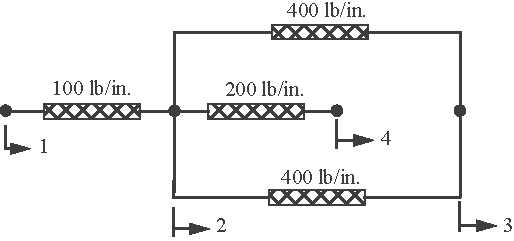
\includegraphics{Figure_15-14.pdf}
}{\caption{Spring model
of example 15.2.\label{fig15.14}}}}


The unrestrained structural stiffness matrix is given as
\begin{align}\label{ex15.2a}
[K]=
\begin{array}{@{}l@{}}
{\arraycolsep=13pt\begin{array}{@{}l@{}}
\hspace*{12pt}q_{1} \hspace*{25pt} q_{2} \hspace*{22pt} q_{3} \hspace*{22pt} q_{4}
\end{array}}\\[4pt]
\left[\begin{array}{@{}cccc@{}} 100 & -100 & 0 & 0 \\-100 & 1,100 & -800 & -200 \\0 & -800 & 800 & 0 \\0 & -200 & 0 & 200\end{array}\right]
\end{array}\,\mathrm{lb.}/\text{in.}
\end{align}
It is prescribed that the displacement $q_1 = 1$ in., force ${Q}_2 = 0$, force ${Q}_3 = –400$~lb., and that the displacement ${q_4 = 0}$.
\begin{enumerate}[b)]\leftskip13pt
  \item[{\hskip13pt}a)] Determine the nodal displacement vectors $\{q_{\alpha}\}$ and $\{q_{\beta}\}$, and the nodal force vectors $\{Q_{\alpha}\}$ and $\{Q_{\beta}\}$.
  \item[{\hskip13pt}b)] Determine the submatrices $[K_{\alpha \alpha}],[K_{\alpha \beta}],[K_{\beta \alpha}]$, and $\left[K_{\beta \beta}\right]$.
  \item[{\hskip13pt}c)] Solve for the unknown nodal displacements and forces.
\end{enumerate}

\subsubsection{Solution to part (a).} The known and unknown quantities are listed in table \ref{tab15.1}
\setcounter{equation}{3}
\begin{table}[h]
\processtable{Classification of the nodal quantities\label{tab15.1}}{%
\tabcolsep=30pt\begin{tabular}{@{}l|llll@{}}
\hline
%\toprule
&&&&\\[-9pt]
\colhead{Known} &   \colhead{${q_{\bf 1}}$} & \colhead{${Q}_{\bf 2}$} & \colhead{${Q}_{\bf 3}$} & \colhead{$q_{\bf 4}$}\\
&&&&\\[-9pt]
\hline
&&&&\\[-9pt]
%\midrule
Unknown & ${Q}_1$ & $q_2$ & $q_3$ & ${{Q}_4}_{\vphantom{T}}$\\
%\botrule
&&&&\\[-9pt]
\hline
\end{tabular}}{}
\end{table}

\noindent Therefore, the $\alpha$-indices are 2 and 3, and the $\beta$-indices are 1 and 4. The unknown nodal displacement vector and the corresponding known nodal force vector are
\begin{align}\label{ex15.2d}
\{q_{\alpha}\}=\left[\begin{array}{@{}l@{}}q_{2} \\q_{3}\end{array}\right] \quad\{Q_{\alpha}\}=\left[\begin{array}{@{}l@{}}Q_{2} \\Q_{3}\end{array}\right]=\left[\begin{array}{@{}c@{}}0 \\-400\end{array}\right].
\end{align}
The known displacement vector and the corresponding unknown force vector are
\begin{align}\label{ex15.2e}
\{q_{\beta}\}=\left[\begin{array}{@{}l@{}}q_{1} \\q_{4}\end{array}\right]=\left[\begin{array}{@{}l@{}}1 \\0\end{array}\right] \quad\{Q_{\beta}\}=\left[\begin{array}{@{}l@{}}Q_{1} \\Q_{4}\end{array}\right].
\end{align}

\subsubsection{Solution to part (b).} We change the order of the columns in the unrestrained structural stiffness matrix to correspond to displacements $q_2$, $q_3$, $q_1$, and $q_4$. Simultaneously we change the order of the rows to correspond to forces ${Q}_2$, ${Q}_3$, ${Q}_1$, and ${Q}_4$. The re-ordered unrestrained structural stiffness matrix is
\begin{align}\label{ex15.2f}
\begin{array}{cc@{}}
 \begin{array}{c@{}}
Q_{2}: \\
Q_{3}: \\
Q_{1}:\\
Q_{4}:
\end{array}
&
\begin{array}{@{}l@{}}
{\arraycolsep=13pt\begin{array}{@{}l@{}}
\hspace*{12pt}q_{2} \hspace*{25pt} q_{3} \hspace*{22pt} q_{1} \hspace*{22pt} q_{4}
\end{array}}\\[4pt]
\left[
\begin{array}{@{\ }cc;{2pt/2pt}cc@{\ }}
1{,}100 & -800 & -100 & -200 \\ -800 & 800 & 0 & 0 \\\hdashline[2pt/2pt]
-100 & 0 & 100 & 0 \\  -200 & 0 & 0 & 200
\end{array}
\right]
\end{array}
\end{array}.
\end{align}

Compare the partition form of the previous matrix to the general partitioned form given by eq.~(\ref{eq15.27}) to find
\begin{equation}\label{ex15.2g}
\begin{split}
&[K_{\alpha \alpha}]=\left[\begin{array}{@{}cc@{}}1{,}100 & -800 \\-800 & 800\end{array}\right] \qquad\left[K_{\alpha \beta}\right]=\left[\begin{array}{@{}cc@{}}-100 & -200 \\0 & 0\end{array}\right]\\
&[K_{\beta \alpha}]=\left[\begin{array}{@{}ll@{}}-100 & 0 \\-200 & 0\end{array}\right]
\qquad \left[K_{\beta \beta}\right]=\left[\begin{array}{@{}cc@{}}100 & 0 \\0 & 200\end{array}\right]
\end{split}.
\end{equation}

\enlargethispage{-2\baselineskip}

\subsubsection{Solution to part (c).} The general form for the solution to the unknown nodal displacement vector is given by eq.~(\ref{eq15.33}). For this example the general form of the solution becomes
\begin{align}\label{ex15.2h}
\left[\begin{array}{@{}l@{}}q_{2} \\q_{3}\end{array}\right]=\left[\begin{array}{@{}cc@{}}1,100 & -800 \\-800 & 800\end{array}\right]^{-1}\left[\begin{array}{@{}c@{}}0 \\-400\end{array}\right]-\left[\begin{array}{@{}cc@{}}1,100 & -800 \\-800 & 800\end{array}\right]^{-1}\left[\begin{array}{@{}cc@{}}-100 & -200 \\0 & 0\end{array}\right]\left[\begin{array}{@{}l@{}}1 \\0\end{array}\right]=\left[\begin{array}{@{}c@{}}-1 \\-1.5\end{array}\right] \text{ in. }.
\end{align}
Since the nodal displacement vector $\{q_{\alpha}\}$ has been determined, we use eq.~(\ref{eq15.32}) to find the unknown nodal force vector; i.e.,
\begin{align}\label{ex15.2i}
\left[\begin{array}{@{}l@{}}Q_{1} \\Q_{4}\end{array}\right]=\left[\begin{array}{@{}ll@{}}-100 & 0 \\-200 & 0\end{array}\right]\left[\begin{array}{@{}c@{}}-1 \\-1.5\end{array}\right]+\left[\begin{array}{@{}cc@{}}100 & 0 \\0 & 200 \end{array}\right]\left[\begin{array}{@{}l@{}}1 \\0\end{array}\right]=\left[\begin{array}{@{}l@{}}200 \\200\end{array}\right]1\textrm{b}.
\end{align}
\hfill\qed
\end{example*}

\begin{thebibliography}{}\label{sec15.8}
\bibitem{}
Martin, Harold C. \textit{\textbf{Introduction to Matrix Methods of Structural Analysis}}. New York: McGraw-Hill Book Company, 1966.
\end{thebibliography}

\pagebreak


\section{Practice exercises}\label{sec15.9}

\begin{exercise}
\begin{enumerate}[\textbf{2.}]
\item[\textbf{1.}] For the spring assembly shown in figure \ref{fig15.15}, determine the 2X2 flexibility influence matrix $[C]$ by the method of unit action states.

    {\def\thefigure{15.15}
\processfigure{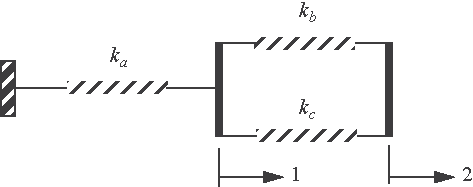
\includegraphics{Figure_15-15.pdf}
}{\caption{Spring assembly of exercise 1.\label{fig15.15}}}}


\item[\textbf{2.}] Consider a three-degree-of-freedom model of the string in tension shown in figure \ref{fig15.16}. Let $T$ denote the horizontal component of the tension force. The three degrees of freedom are the vertical displacements and corresponding forces at the quarter points. The analysis of this structure is different from the analyses we have been using in that \textit{we have to take equilibrium on a slightly deflected configuration rather than on the undeformed configuration even though the displacements are small.} A typical free body diagram to be used in the analysis is shown in the figure. Note that it is the horizontal component of the string tension that is equal to $T$.

 {\def\thefigure{15.16}
\processfigure{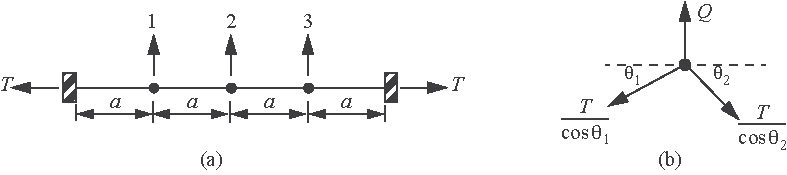
\includegraphics{Figure_15-16.pdf}
}{\caption{(a) String in tension. (b) Typical free body diagram.\label{fig15.16}}}}

\enlargethispage{-2\baselineskip}

\begin{enumerate}[b)]
  \item[{\hskip13pt}a)] Use unit action states and the physical definition of flexibility influence coefficients to calculate the 3X3 flexibility matrix $[C]$. Write the elements of the matrix in terms of tension $T$ and dimension $a$. Recall the vertical displacements are assumed small compared to length $a$. Partial answer: $c_{11}=\frac{3}{4}\left(\frac{a}{T}\right)$.
  \item[{\hskip13pt}b)] Use unit displacement states and the physical definition of stiffness matrix elements to calculate the 3X3 stiffness matrix $[K]$. Partial answer: $k_{11}=2\left(\frac{T}{a}\right)$.
  \item[{\hskip13pt}c)] Check the plausibility of the matrices determined in parts \textbf{a} and \textbf{b}. Are they symmetric? Are diagonal elements positive? Does $[K][C]=[I]$?
\end{enumerate}

\item[\textbf{3.}] Derive by the method of unit displacement states the 3X3 stiffness matrix $[K]$ for the structure shown in figure \ref{fig15.17}. Assume small displacements and rotations of the horizontal rigid bar. Partial answer: $k_{21}=2 k/9$.

 {\def\thefigure{15.17}
\processfigure[H]{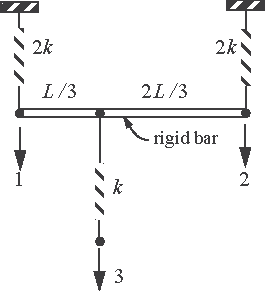
\includegraphics{Figure_15-17.pdf}
}{\caption{Exercise 3.\label{fig15.17}}}}


\item[\textbf{4.}] For the spring model in example \ref{fig15.2}, use eq.~(\ref{eq15.45}) and determine the stress matrix and spring force in spring elements 1-2, 2-3, and 2-4. State if the spring element is in tension or compression. Note: the spring force 2-3 is the force in the upper and lower spring between joints 2 and 3.
\end{enumerate}
\end{exercise}

\end{document} 